\section{Complete Experimental Results Table}
\label{sec:vmg}

\begin{table}[H]
\centering
\footnotesize
\setlength{\tabcolsep}{3.5pt}
\renewcommand{\arraystretch}{0.88}
\begin{tabular}{@{}rr rrr rrr rrr@{}}
\toprule
& & \multicolumn{3}{c}{\textbf{MLP}} & \multicolumn{3}{c}{\textbf{PID}} & \multicolumn{3}{c}{\textbf{1DCNN (This work)}} \\
\cmidrule(lr){3-5} \cmidrule(lr){6-8} \cmidrule(lr){9-11}
Hdg ($^\circ$) & Wind (kt) & CMG & Err ($^\circ$) & XTE (m) & CMG & Err ($^\circ$) & XTE (m) & CMG & Err ($^\circ$) & XTE (m) \\
\midrule
85  & 10 &  9.44 & 10.40 & 155.12 & 10.95 & 1.25 & 21.31 & \textcolor{red}{11.53} &  6.10 & 108.46 \\
85  & 14 & 16.67 &  0.60 &  15.41 & 16.51 & 1.54 & 39.66 & \textcolor{red}{17.23} &  3.75 & 100.85 \\
85  & 18 & 19.35 &  2.39 &  72.49 & 19.62 & 0.94 & 28.84 & \textcolor{red}{19.99} &  0.99 &  30.94 \\
85  & 20 & 22.19 &  4.65 & 162.10 & 23.11 & 1.05 & 38.08 & \textcolor{red}{23.50} &  0.88 &  32.36 \\
\midrule
95  & 10 &  9.49 & 11.90 & 179.37 & 11.00 & 1.32 & 22.67 & \textcolor{red}{11.04} & 15.58 & 283.57 \\
95  & 14 & 16.59 &  0.62 &  15.95 & 16.48 & 1.55 & 39.78 & \textcolor{red}{17.02} &  3.95 & 105.38 \\
95  & 18 & 20.35 &  1.70 &  54.21 & 20.40 & 0.97 & 30.99 & \textcolor{red}{20.54} &  0.02 &   0.58 \\
95  & 20 & 23.24 &  4.61 & 168.55 & 23.87 & 1.10 & 40.94 & \textcolor{red}{24.59} &  7.71 & 299.62 \\
\midrule
115 & 10 & \textcolor{red}{10.14} &  6.57 & 104.95 &  9.94 & 1.47 & 22.78 & N/A   & N/A   & N/A    \\
115 & 14 & 14.00 & 11.88 & 266.68 & \textcolor{red}{15.05} & 1.54 & 36.16 & 14.98 &  2.01 &  48.00 \\
115 & 18 & 20.42 &  2.07 &  66.18 & 20.50 & 1.08 & 34.57 & \textcolor{red}{20.53} &  7.10 & 230.81 \\
115 & 20 & 24.00 &  5.56 & 209.87 & \textcolor{red}{24.36} & 1.18 & 44.99 & 23.99 &  7.92 & 302.95 \\
\midrule
135 & 10 &  8.39 & 10.32 & 137.14 & \textcolor{red}{8.71} & 1.64 & 22.26 & N/A   & N/A   & N/A    \\
135 & 14 & 11.49 & 19.33 & 363.91 & \textcolor{red}{12.83} & 1.61 & 32.11 & 12.53 &  0.41 &   7.74 \\
135 & 18 & 17.05 & 11.39 & 309.64 & 17.64 & 1.06 & 29.34 & \textcolor{red}{17.65} &  0.15 &   3.38 \\
135 & 20 & \textcolor{red}{19.77} &  2.07 &  63.96 & 19.76 & 1.08 & 33.37 & 19.39 &  4.49 & 137.72 \\
\midrule
145 & 10 &  6.95 & 11.90 & 132.60 & \textcolor{red}{8.23} & 1.76 & 22.41 & N/A   & N/A   & N/A    \\
145 & 14 &  9.89 & 22.01 & 360.30 & \textcolor{red}{11.81} & 1.69 & 30.97 & 11.56 &  7.62 & 138.39 \\
145 & 18 & 13.49 & 23.97 & 546.05 & \textcolor{red}{15.85} & 1.13 & 27.78 & 15.84 &  2.86 &  70.94 \\
145 & 20 & 15.66 & 18.04 & 463.74 & \textcolor{red}{17.55} & 1.08 & 29.46 & 17.47 &  0.20 &   5.49 \\
\bottomrule
\end{tabular}
\caption{Systematic comparison of navigational metrics across architectural groups, sorted by heading and wind intensity.}
\label{tab:results_sorted}
\end{table}

\section{CMG Improvement Over Baseline}
\label{sec:cmg_improvement}

\begin{table}[htbp]
\centering
\footnotesize
\setlength{\tabcolsep}{5pt}
\renewcommand{\arraystretch}{0.92}
\begin{tabular}{@{}rr rrr rr@{}}
\toprule
& & \multicolumn{3}{c}{\textbf{CMG Values}} & \multicolumn{2}{c}{\textbf{\% Improvement vs PID}} \\
\cmidrule(lr){3-5} \cmidrule(lr){6-7}
Hdg ($^\circ$) & Wind (kt) & MLP & PID & 1DCNN & MLP & 1DCNN \\
\midrule
85  & 10 &  9.44 & 10.95 & 11.53 & $-13.77$ & \textcolor{red}{$+5.27$} \\
85  & 14 & 16.67 & 16.51 & 17.23 & \textcolor{red}{$+0.92$}  & \textcolor{red}{$+4.33$} \\
85  & 18 & 19.35 & 19.62 & 19.99 & $-1.36$  & \textcolor{red}{$+1.90$} \\
85  & 20 & 22.19 & 23.11 & 23.50 & $-3.95$  & \textcolor{red}{$+1.72$} \\
\midrule
95  & 10 &  9.49 & 11.00 & 11.04 & $-13.71$ & \textcolor{red}{$+0.36$} \\
95  & 14 & 16.59 & 16.48 & 17.02 & \textcolor{red}{$+0.71$}  & \textcolor{red}{$+3.28$} \\
95  & 18 & 20.35 & 20.40 & 20.54 & $-0.28$  & \textcolor{red}{$+0.67$} \\
95  & 20 & 23.24 & 23.87 & 24.59 & $-2.61$  & \textcolor{red}{$+3.02$} \\
\midrule
115 & 10 & 10.14 &  9.94 & N/A  & \textcolor{red}{$+2.03$} & N/A     \\
115 & 14 & 14.00 & 15.05 & 14.98 & $-6.98$  & $-0.44$  \\
115 & 18 & 20.42 & 20.50 & 20.53 & $-0.39$  & \textcolor{red}{$+0.14$} \\
115 & 20 & 24.00 & 24.36 & 23.99 & $-1.45$  & $-1.48$  \\
\midrule
135 & 10 &  8.39 &  8.71 & N/A  & $-3.73$  & N/A     \\
135 & 14 & 11.49 & 12.83 & 12.53 & $-10.47$ & $-2.35$  \\
135 & 18 & 17.05 & 17.64 & 17.65 & $-3.36$  & \textcolor{red}{$+0.06$} \\
135 & 20 & 19.77 & 19.76 & 19.39 & \textcolor{red}{$+0.07$} & $-1.87$  \\
\midrule
145 & 10 &  6.95 &  8.23 & N/A  & $-15.55$ & N/A     \\
145 & 14 &  9.89 & 11.81 & 11.56 & $-16.25$ & $-2.15$  \\
145 & 18 & 13.49 & 15.85 & 15.84 & $-14.89$ & $-0.07$  \\
145 & 20 & 15.66 & 17.55 & 17.47 & $-10.78$ & $-0.44$  \\
%\midrule
%\multicolumn{5}{@{}r}{\textbf{Average}} & $\mathbf{-5.80}$ & $\mathbf{+0.70}$ \\
%\multicolumn{5}{@{}r}{\textbf{Rows beating PID}} & $\mathbf{3/17}$ & $\mathbf{10/17}$ \\
\bottomrule
\end{tabular}
\caption{Percentage CMG improvement of MLP and 1DCNN over the PID baseline. N/A indicates the model failed for that condition. Positive values (red) indicate the model outperforms PID.}
\label{tab:cmg_improvement}
\end{table}



\section{Complete Trajectory Comparison}
\label{sec:cmg_improvement}

\begin{figure}[H]
    \centering
    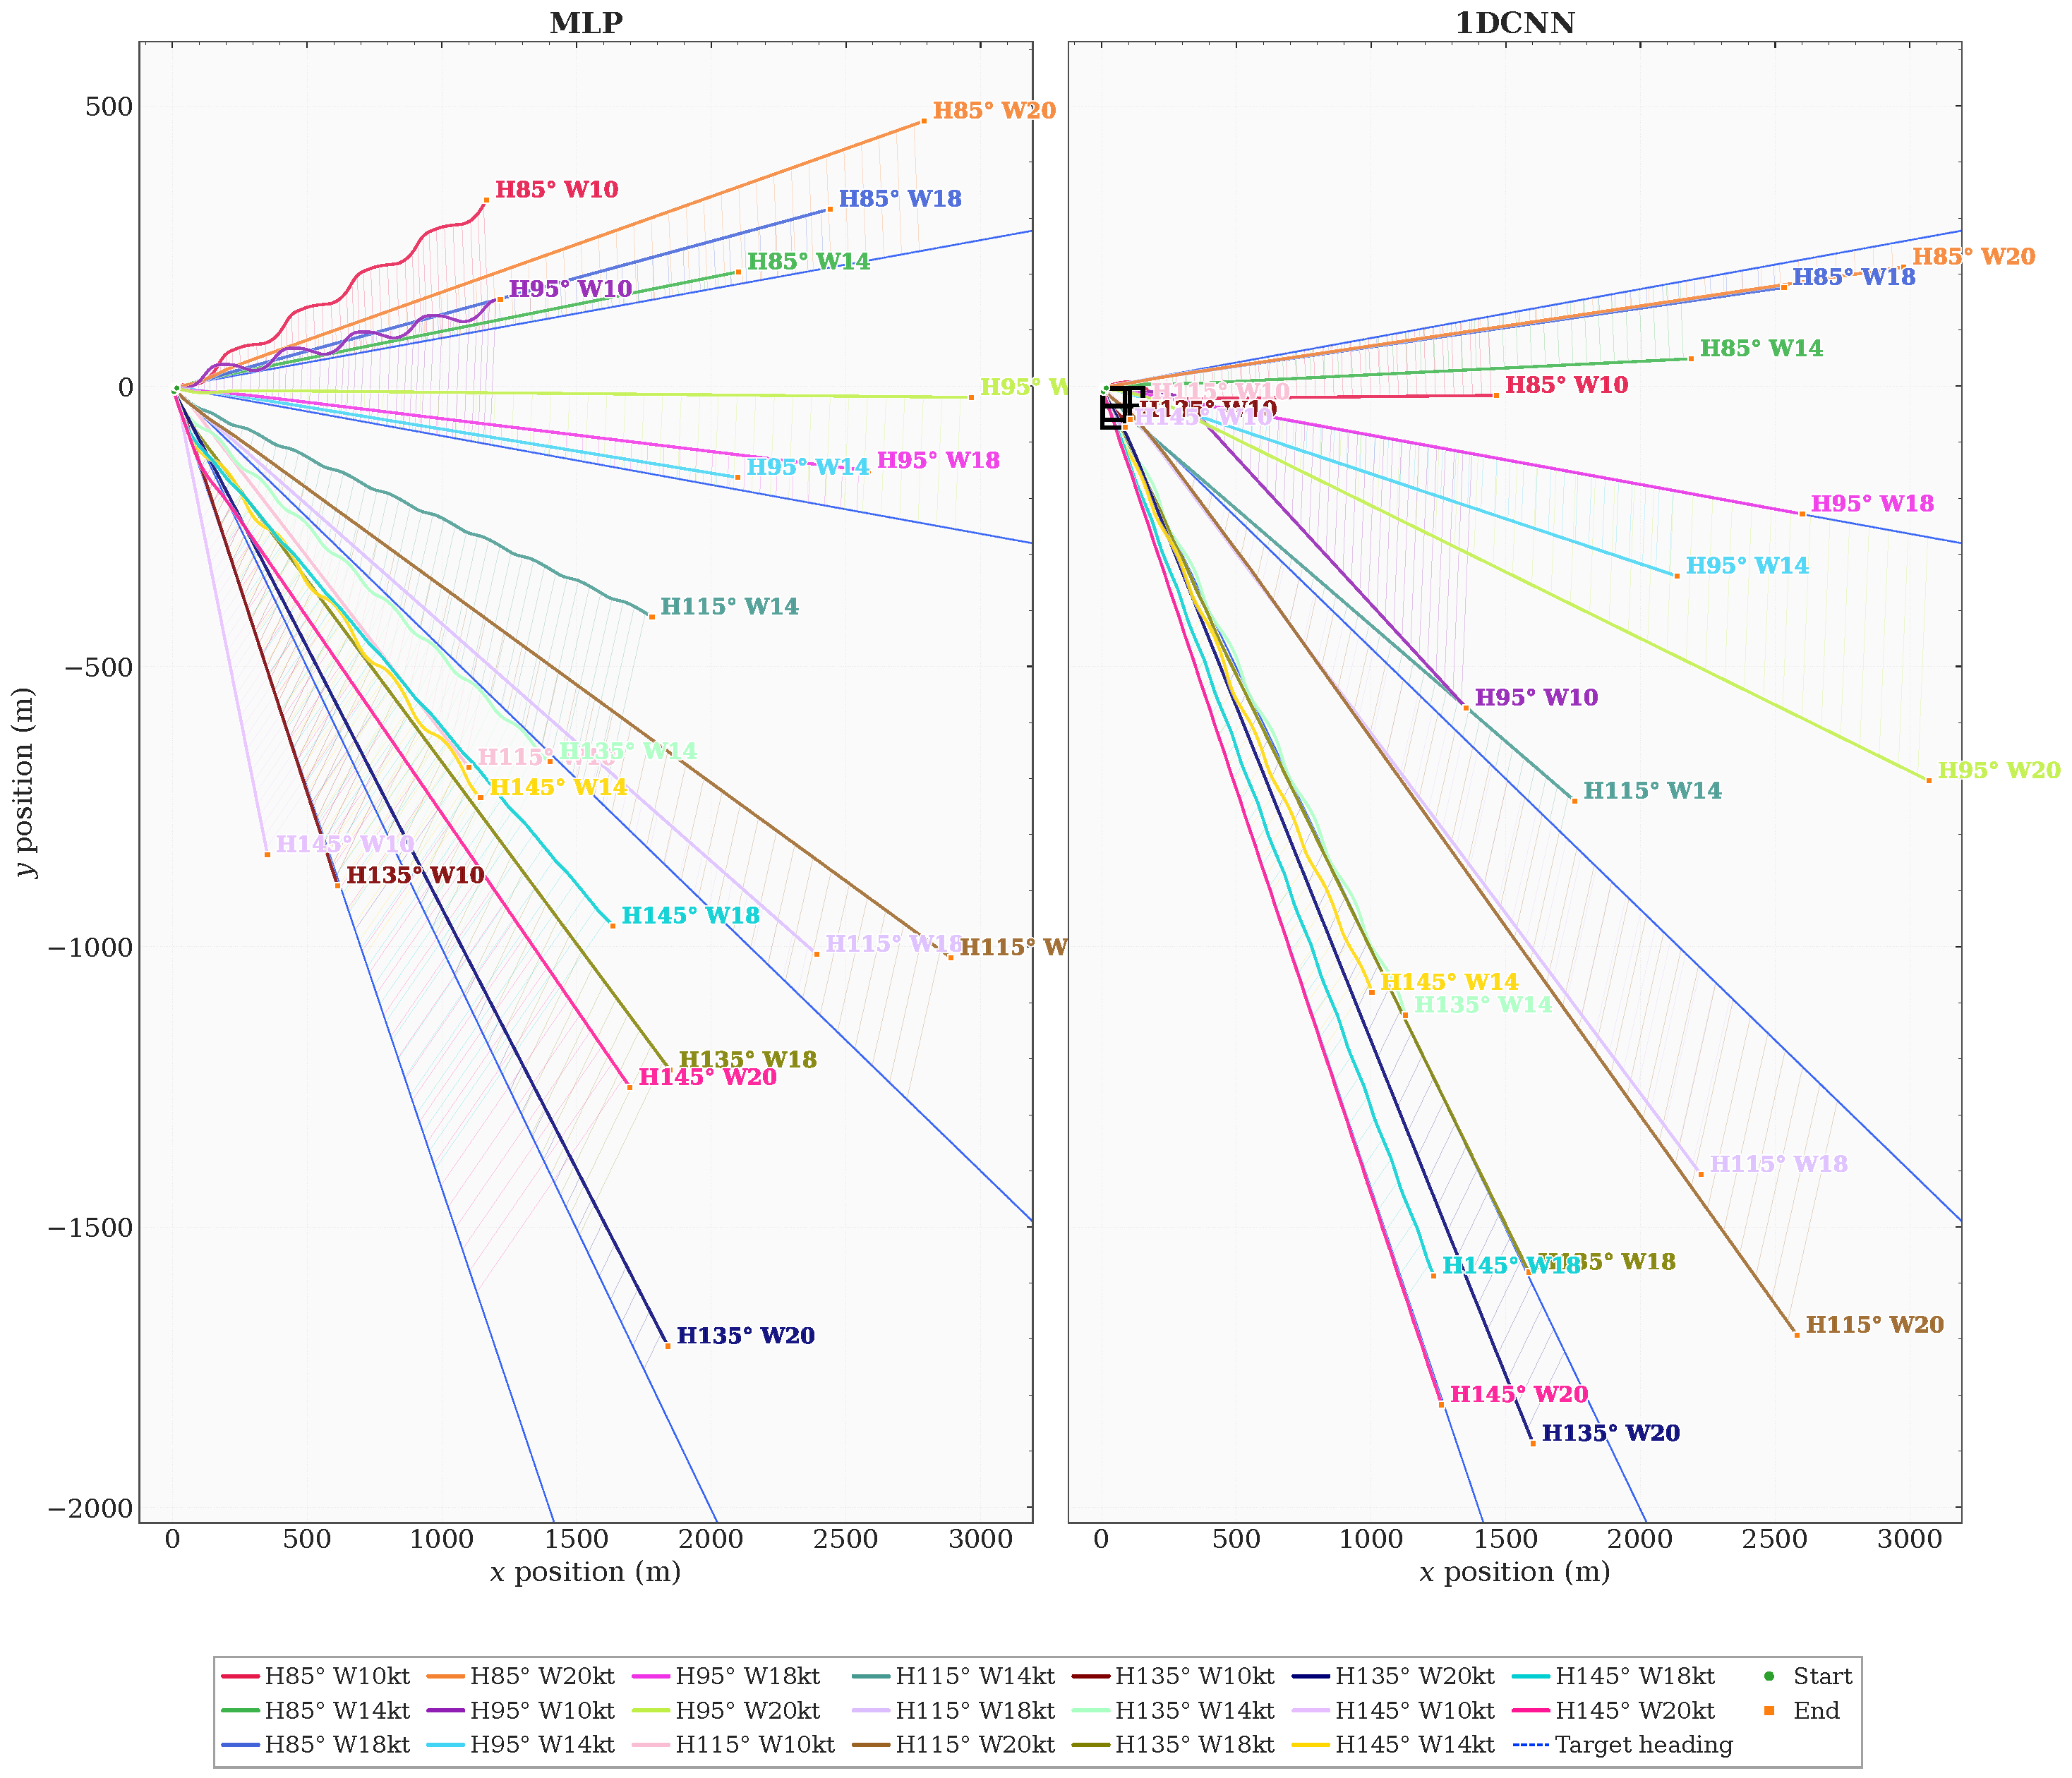
\includegraphics[width=0.8\linewidth]{resources/img/appendix/trajectory_grid_pub.pdf}
    \caption{Trajectory comparison across both architectures under all heading and wind conditions.}
    \label{fig:trajectory_grid}
\end{figure}

\justify
The trajectory plots provide a qualitative comparison of steering behaviors across the evaluation grid. The Baseline controller produces smooth, linear paths but exhibits significant drift under high-wind conditions, indicating limited proactive adaptation. The MLP shows clear instability, particularly at $H:85^\circ \mid W:10\,\text{kt}$, where large oscillations suggest poor damping and reduced navigational efficiency. In contrast, the 1DCNN maintains the most robust trajectories, adhering closely to the intended path even under 20\,kt stress tests. A notable exception arises in light-wind conditions (10\,kt) at headings of $115^\circ$, $135^\circ$, and $145^\circ$, where aggressive micro-corrections occasionally lead to ``Out-of-Bound'' (OOB) terminations. Despite these edge-case failures, the 1DCNN consistently outperforms the other architectures in high-performance foiling scenarios.




